\documentclass[aspectratio=169,11pt]{beamer}
\usepackage[T1]{fontenc}
\usepackage{lmodern,amsmath,amssymb,mathtools,bm,booktabs,array,graphicx,tikz}
\usetikzlibrary{arrows.meta,positioning,calc,decorations.pathreplacing,patterns}
\definecolor{ink}{HTML}{17344D}\definecolor{accent}{HTML}{087E8B}\definecolor{pale}{HTML}{EDF5F5}\definecolor{gold}{HTML}{AD6B19}
\providecommand{\dd}{\,\mathrm{d}}\providecommand{\R}{\mathbb{R}}
\providecommand{\E}{\mathbb{E}}\providecommand{\Var}{\operatorname{Var}}
\providecommand{\Cov}{\operatorname{Cov}}\providecommand{\diag}{\operatorname{diag}}
\providecommand{\norm}[1]{\left\lVert#1\right\rVert}
\providecommand{\abs}[1]{\left|#1\right|}
\usefonttheme{professionalfonts}
\setbeamercolor{normal text}{fg=black,bg=white}
\setbeamercolor{frametitle}{fg=ink,bg=white}
\setbeamercolor{title}{fg=ink}\setbeamercolor{structure}{fg=accent}
\setbeamercolor{block title}{fg=ink,bg=pale}\setbeamercolor{block body}{fg=black,bg=pale!40}
\setbeamercolor{alerted text}{fg=accent}
\setbeamerfont{frametitle}{size=\Large,series=\bfseries}
\setbeamerfont{title}{size=\LARGE,series=\bfseries}
\setbeamertemplate{navigation symbols}{}
\setbeamersize{text margin left=.7cm,text margin right=.7cm}
\setbeamertemplate{frametitle}{\vspace{.18cm}\insertframetitle\par\vspace{.1cm}{\color{accent}\hrule height .6pt}\vspace{.12cm}}
\newcommand{\notestarget}{notes.pdf}\newcommand{\noteslabel}{Notes}
\setbeamertemplate{footline}{\hspace{.7cm}\color{ink}\scriptsize Computational Cardiology\quad\href{\notestarget}{\noteslabel}\hfill\insertframenumber\,/\,\inserttotalframenumber\hspace{.7cm}\vspace{.18cm}}
\setbeamercovered{invisible}
\hypersetup{pdfauthor={Zan Ahmad},pdftitle={Planar viscous flow and boundary-value discretization},pdfpagemode=UseNone}
\begin{document}
\begin{frame}[plain]\vfill
{\small\color{accent} Computational Cardiology \quad Lecture 7}\par\medskip
{\raggedright\hyphenpenalty=10000\exhyphenpenalty=10000\LARGE\bfseries\color{ink} Planar viscous flow and boundary-value discretization}\par\bigskip
Zan Ahmad\par\smallskip
{\small Fall 2024}\par\vfill\end{frame}
\renewcommand{\notestarget}{notes.pdf\#note-incompressibility-and-the-missing-momentum-equation}
\begin{frame}[t,fragile,label=slide-the-incompressible-balance]{The incompressible balance}
\[\nabla\cdot\boldsymbol u=0,\qquad\int_{\partial\Omega}\boldsymbol u\cdot n\,\mathrm dS=0.\]\pause{} These equations constrain volume transport, not its magnitude.
\end{frame}
\renewcommand{\notestarget}{notes.pdf\#note-incompressibility-and-the-missing-momentum-equation}
\begin{frame}[t,fragile,label=slide-a-fully-developed-velocity]{A fully developed velocity}
\[\boldsymbol u=(u(y),0).\]\pause{} Both divergence and convective acceleration vanish for this ansatz. Momentum must still select $u$.
\end{frame}
\renewcommand{\notestarget}{notes.pdf\#note-integration-of-the-reduced-momentum-balance}
\begin{frame}[t,fragile,label=slide-reduced-momentum]{Reduced momentum}
\[\mu u^{\prime\prime}=-G,\qquad G=-\frac{\mathrm dp}{\mathrm dx}.\]\pause{} Positive $G$ drives positive downstream flow.
\end{frame}
\renewcommand{\notestarget}{notes.pdf\#note-integration-of-the-reduced-momentum-balance}
\begin{frame}[t,fragile,label=slide-two-integrations]{Two integrations}
\[u(y)=-\frac{G}{2\mu}y^2+A y+B.\]\pause{} The two constants are fixed by $u(0)=U_0$ and $u(H)=U_H$.
\end{frame}
\renewcommand{\notestarget}{notes.pdf\#note-integration-of-the-reduced-momentum-balance}
\begin{frame}[t,fragile,label=slide-the-couette-poiseuille-profile]{The Couette--Poiseuille profile}
\[u(y)=\frac{G}{2\mu}y(H-y)+U_0+\frac{U_H-U_0}{H}y.\]\pause{} The pressure-driven quadratic and wall-driven linear profiles superpose.
\end{frame}
\renewcommand{\notestarget}{notes.pdf\#note-pressure-driven-and-moving-wall-flow}
\begin{frame}[t,fragile,label=slide-flux-and-maximum-speed]{Flux and maximum speed}
For stationary walls,\[u_{\max}=\frac{GH^2}{8\mu},\qquad q=\frac{GH^3}{12\mu},\qquad Q=Wq.\]\pause{} $q$ has units m$^2$/s; $Q$ has units m$^3$/s.
\end{frame}
\renewcommand{\notestarget}{notes.pdf\#note-pressure-driven-and-moving-wall-flow}
\begin{frame}[label=slide-a-synthetic-channel-figure]{Boundary values determine the velocity profile}
\centering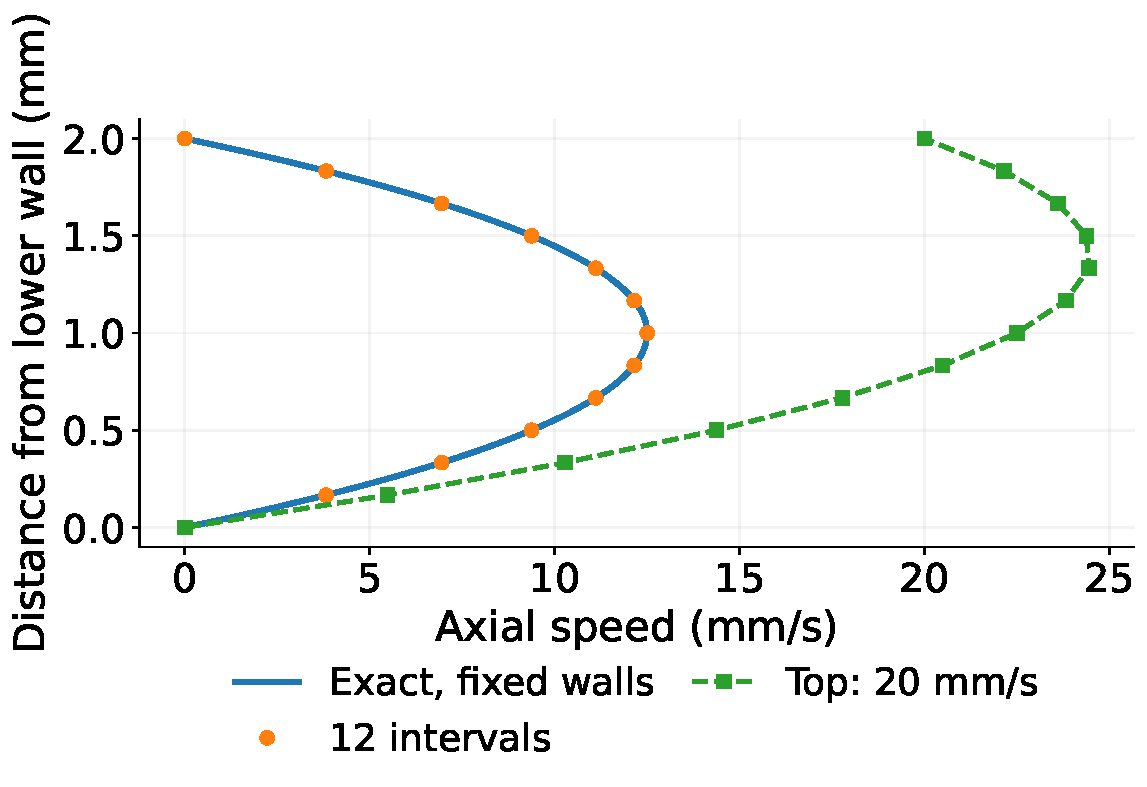
\includegraphics[width=.98\linewidth,height=.69\textheight,keepaspectratio]{presentation-figures/channel-profiles-panel-1.pdf}\end{frame}
\renewcommand{\notestarget}{notes.pdf\#note-pressure-driven-and-moving-wall-flow}
\begin{frame}[t,fragile,label=slide-a-synthetic-channel]{A synthetic channel}
\[H=.002\ \mathrm m,\quad \mu=.004\ \mathrm{Pa\,s},\quad G=100\ \mathrm{Pa/m}.\]\pause{}\[u_{\max}=.0125\ \mathrm{m/s},\qquad q=1.6667\times10^{-5}\ \mathrm{m^2/s}.\]
\end{frame}
\renewcommand{\notestarget}{notes.pdf\#note-pressure-driven-and-moving-wall-flow}
\begin{frame}[t,fragile,label=slide-hydraulic-resistance-of-the-planar-channel]{Hydraulic resistance of the planar channel}
\[\Delta p=GL,\qquad R=\frac{\Delta p}{Q}=\frac{12\mu L}{WH^3}.\]\pause{} The gap dependence follows from this geometry.
\end{frame}
\renewcommand{\notestarget}{notes.pdf\#note-the-discrete-dirichlet-problem}
\begin{frame}[t,fragile,label=slide-centered-interior-equations]{Centered interior equations}
\[2u_j-u_{j-1}-u_{j+1}=\frac{Gh^2}{\mu},\qquad h=H/N.\]\pause{} Known wall values move to the right-hand side.
\end{frame}
\renewcommand{\notestarget}{notes.pdf\#note-the-discrete-dirichlet-problem}
\begin{frame}[t,fragile,label=slide-the-dirichlet-matrix-is-positive-definite]{The Dirichlet matrix is positive definite}
\[z^{\mathsf T}Az=\sum_{j=0}^{N-1}(z_{j+1}-z_j)^2.\]\pause{} With zero endpoints, equality requires $z=0$.
\end{frame}
\renewcommand{\notestarget}{notes.pdf\#note-exact-nodal-values-and-inexact-quadrature}
\begin{frame}[t,fragile,label=slide-exact-differentiation-of-a-quadratic]{Exact differentiation of a quadratic}
\[\frac{u(y-h)-2u(y)+u(y+h)}{h^2}=u^{\prime\prime}(y)\] for quadratic $u$.\pause{} This benchmark can have roundoff-level nodal error at every grid size.
\end{frame}
\renewcommand{\notestarget}{notes.pdf\#note-exact-nodal-values-and-inexact-quadrature}
\begin{frame}[label=slide-the-integral-is-a-separate-operation-figure]{An exact nodal profile can have an inexact integral}
\centering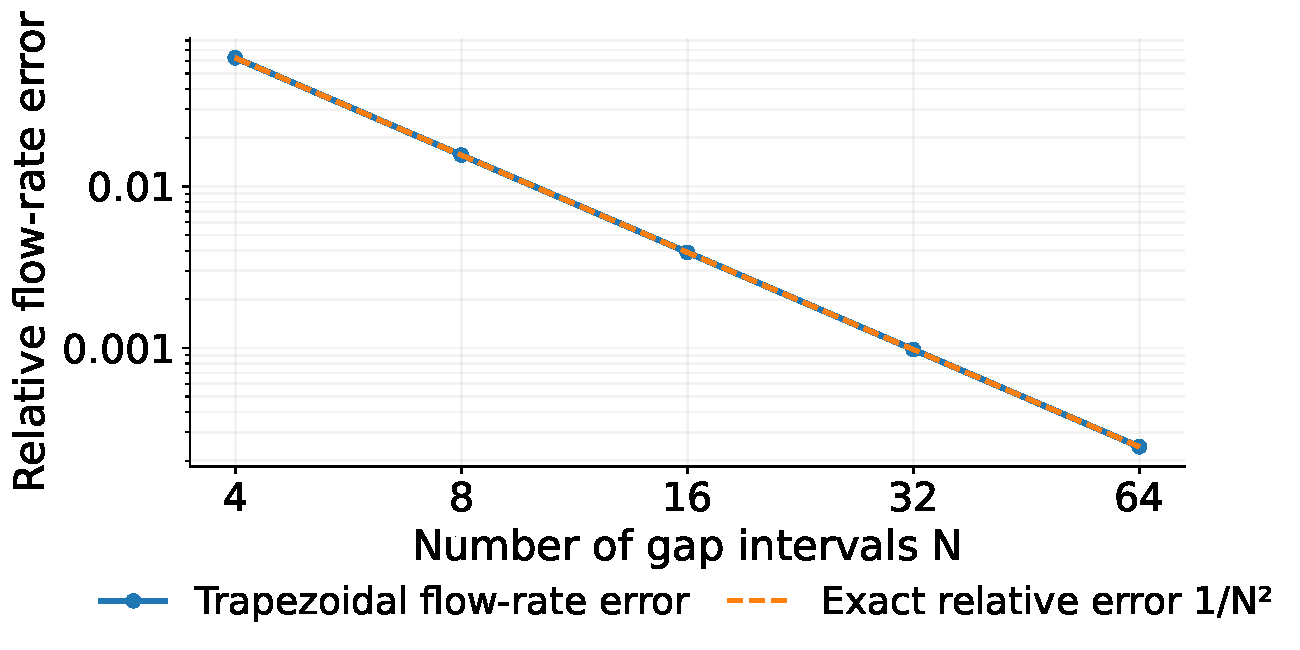
\includegraphics[width=.98\linewidth,height=.69\textheight,keepaspectratio]{presentation-figures/channel-flux-error-panel-1.pdf}\end{frame}
\renewcommand{\notestarget}{notes.pdf\#note-exact-nodal-values-and-inexact-quadrature}
\begin{frame}[t,fragile,label=slide-the-integral-is-a-separate-operation]{The integral is a separate operation}
\[q_h=h\left[\frac{u_0+u_N}{2}+\sum_{j=1}^{N-1}u_j\right].\]\pause{} Straight segments under a concave parabola underestimate its area.
\end{frame}
\renewcommand{\notestarget}{notes.pdf\#note-exact-nodal-values-and-inexact-quadrature}
\begin{frame}[t,fragile,label=slide-an-exact-quadrature-error-formula]{An exact quadrature-error formula}
\[q_h=q(1-N^{-2}),\qquad\frac{q-q_h}{q}=N^{-2}.\]\pause{} The observed order two belongs to quadrature, not a measured nodal-solve error.
\end{frame}
\renewcommand{\notestarget}{notes.pdf\#note-linearity-boundary-data-and-physical-scope}
\begin{frame}[t,fragile,label=slide-changing-the-wall-velocity]{Changing the wall velocity}
\[q=\frac{GH^3}{12\mu}+\frac H2(U_0+U_H).\]\pause{} Trapezoidal quadrature integrates the linear contribution exactly.
\end{frame}
\renewcommand{\notestarget}{notes.pdf\#note-linearity-boundary-data-and-physical-scope}
\begin{frame}[t,fragile,label=slide-the-limits-of-the-reduction]{The limits of the reduction}
The calculation assumes a long straight channel, fixed viscosity and fully developed flow.\pause{} It does not solve an entrance region, moving curved boundaries or general pressure--velocity coupling.
\end{frame}
\end{document}
